% !TEX encoding = UTF-8
% !TEX TS-program = pdflatex
% !TEX root = ../Tesi.tex
% !TEX spellcheck = en-EN

%************************************************
\chapter{Blast Furnace}
\label{cap:blastfurnace}
%************************************************

\info{incomplete}

The raceway, a critical portion of the blast furnace (Fig.
\ref{fig:068racewaylayout}), was investigated.
We performed a limited number of simulations of this volume to investigate the
effect of the variation of input velocity.\\
The results presented in Fig. \ref{fig:068racewaylayout}, Fig.
\ref{fig:225racewayu}, Fig. \ref{fig:238racewayus}, and Fig.
\ref{fig:239racewayvf} were later compared with the literature data from
\citet{RefWorks:208}.

\begin{figure}[!htb]
\centering
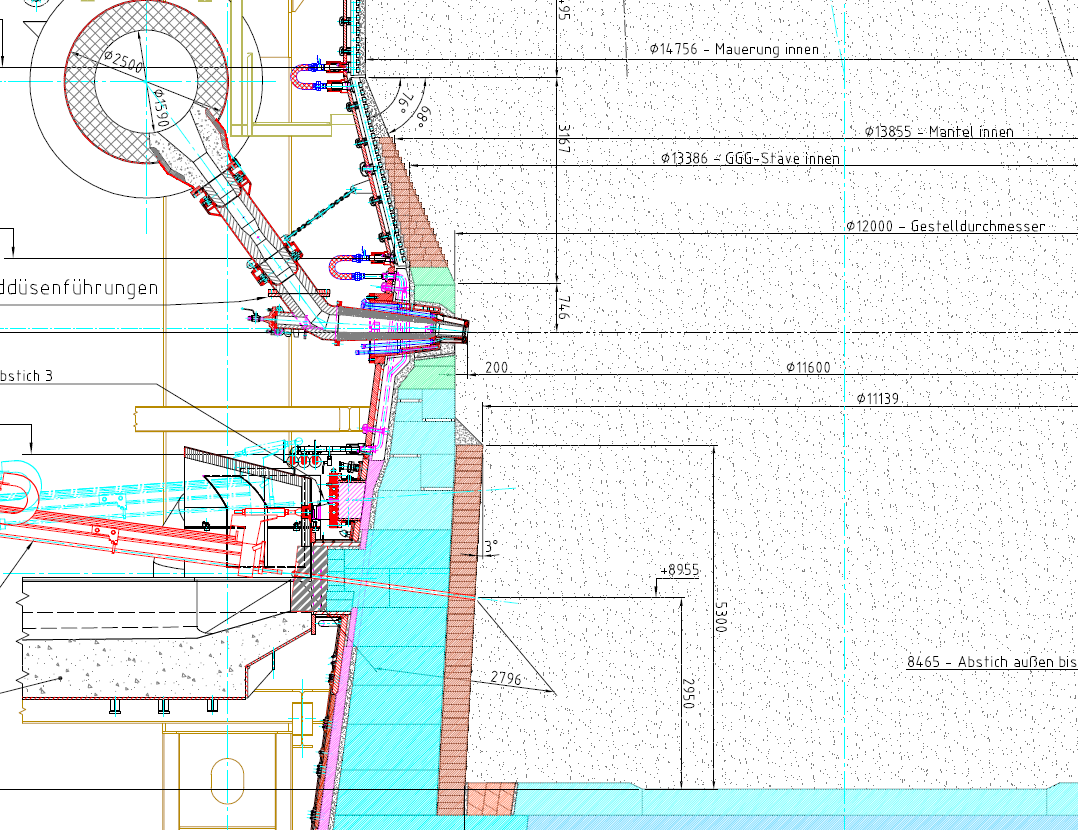
\includegraphics[width=.80\columnwidth]{images/068racewaylayout}
\caption[Blast furnace section layout]{Blast furnace section layout (Voestalpine Stahl GmbH).}
\label{fig:068racewaylayout}
\end{figure}

\newpage

\section{Results}
\label{sec:resultsbf}

The change of sliding friction coefficient bears no effect on the velocity of
the gases. 
Their exit path is clearly accessible and the same kinetic energy, and thus velocity, was
dissipated to displace particles, see Fig. \ref{fig:225racewayu}.\\
However, the particles velocity is clearly, and logically, higher for low
friction particles. They could be moved by the flow more easily compared to high
friction particles, see Fig. \ref{fig:238racewayus}.\\
Concerning the void fraction, low friction allowed a better compaction of the
particles in the top volume, see Fig. \ref{fig:239racewayvf}.
Consequently, the gases need to travel less to reach the top empty volume.
The volume interested by an higher void fraction as effect of the raceway is
thus smaller.	 

\begin{sidewaysfigure}[htbp]
\centering 
  \subfloat[Low friction, average velocity.]
  {
	  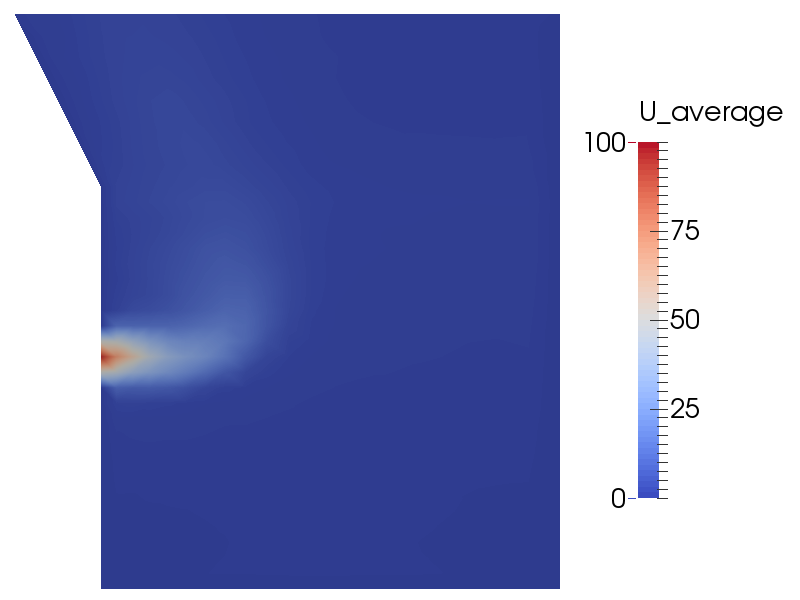
\includegraphics[width=.32\columnwidth]{images/227u_average_lf}
	  \label{fig:227u_average_lf}
  }
  \quad
    \subfloat[High friction, average velocity.]
    {
	  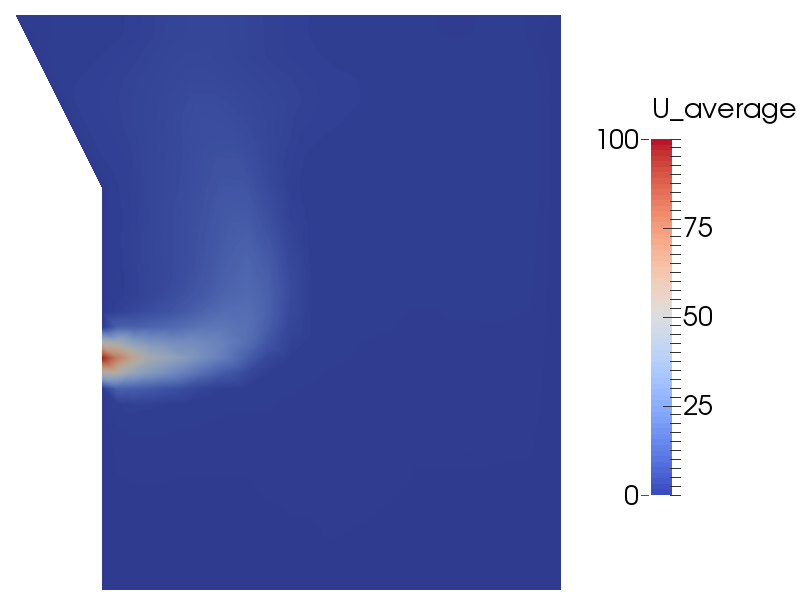
\includegraphics[width=.32\columnwidth]{images/226u_average_hf}
	  \label{fig:226u_average_hf}
  }
  \quad
    \subfloat[High friction, average velocity.]
    {
	  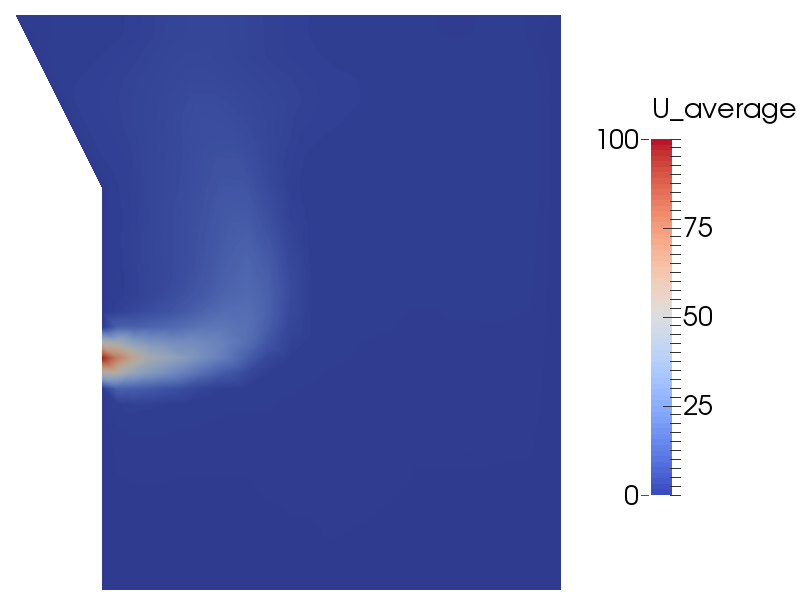
\includegraphics[width=.32\columnwidth]{images/226u_average_hf}
	  \label{fig:226u_average_hf}
  }
  \\
  \subfloat[Low friction, standard deviation velocity.]
  {
	  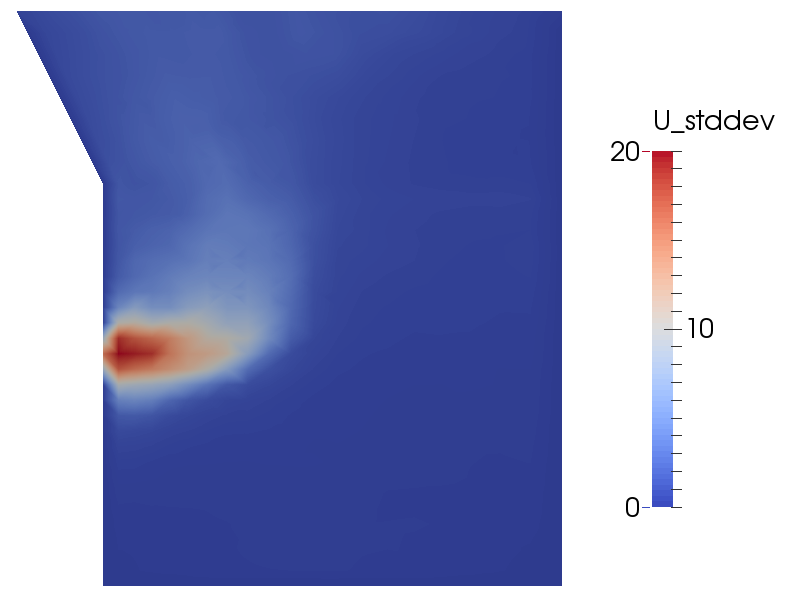
\includegraphics[width=.32\columnwidth]{images/229u_std_lf}
	  \label{fig:229u_std_lf}
  }
  \quad
    \subfloat[High friction, standard deviation velocity.]
    {
	  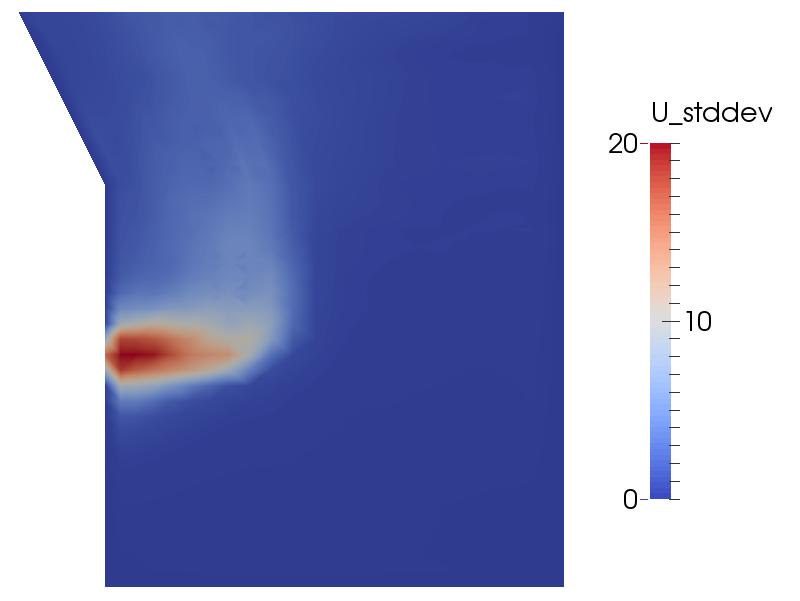
\includegraphics[width=.32\columnwidth]{images/228u_std_hf}
	  \label{fig:228u_std_hf}  }
  \\
  \caption{Fluid velocity with different sliding friction coefficient.}
  \label{fig:225racewayu}
\end{sidewaysfigure}
\begin{sidewaysfigure}[htbp]
\centering 
  \subfloat[Low friction, average velocity.]
  {
	  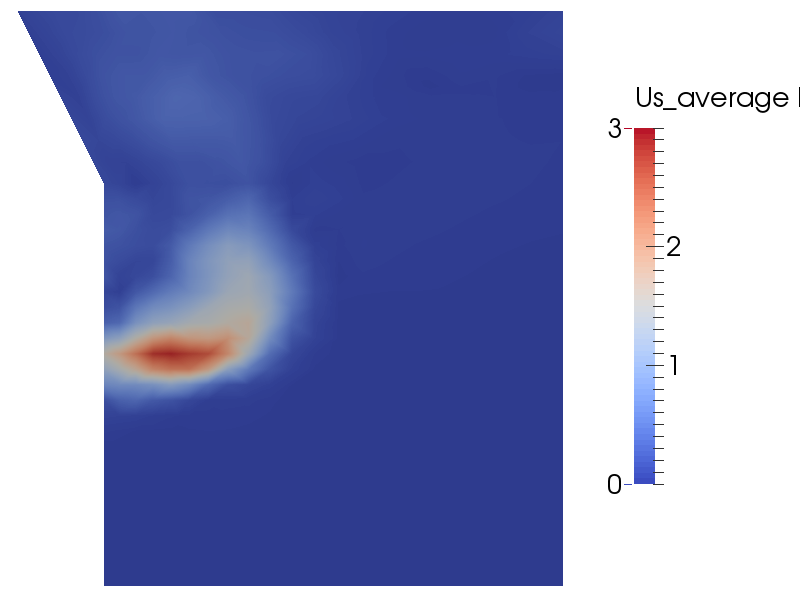
\includegraphics[width=.32\columnwidth]{images/231us_average_lf}
	  \label{fig:231us_average_lf}
  }
  \quad
    \subfloat[High friction, average velocity.]
    {
	  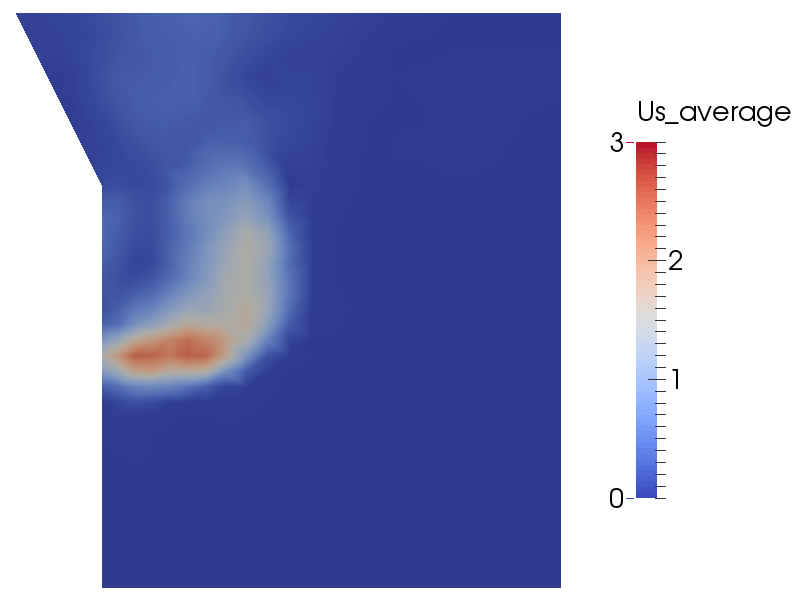
\includegraphics[width=.32\columnwidth]{images/230us_average_hf}
	  \label{fig:230us_average_hf}
  }
  \quad
    \subfloat[High friction, average velocity.]
    {
	  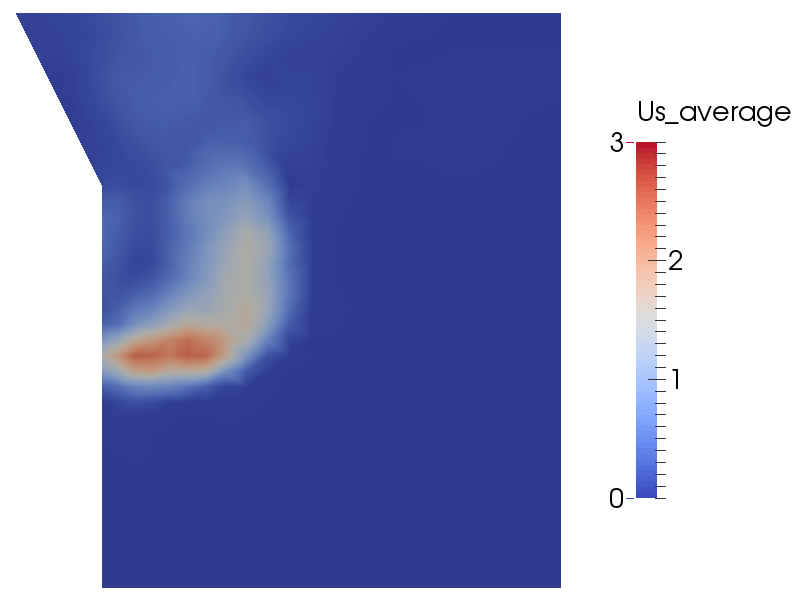
\includegraphics[width=.32\columnwidth]{images/230us_average_hf}
	  \label{fig:230us_average_hf}
  }
  \\
  \subfloat[Low friction, standard deviation velocity.]
  {
	  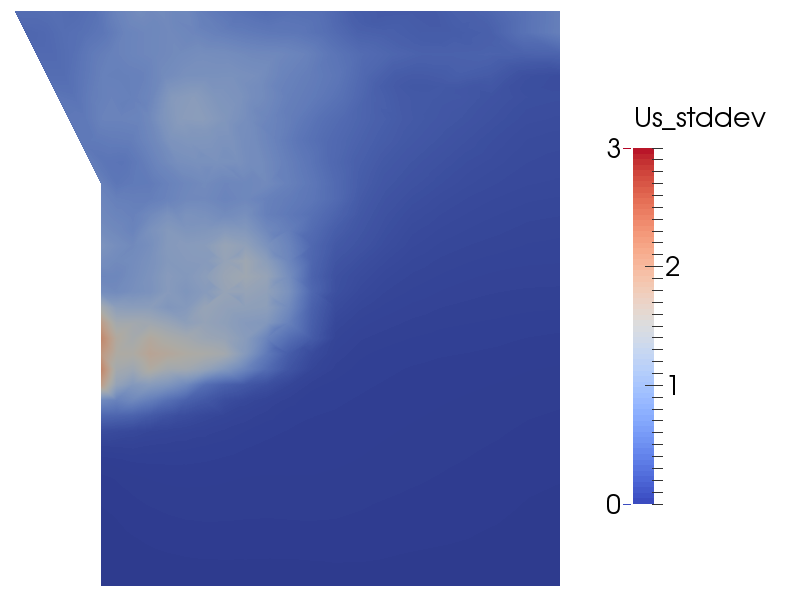
\includegraphics[width=.32\columnwidth]{images/233us_std_lf}
	  \label{fig:233us_std_lf}
  }
  \quad
    \subfloat[High friction, standard deviation velocity.]
    {
	  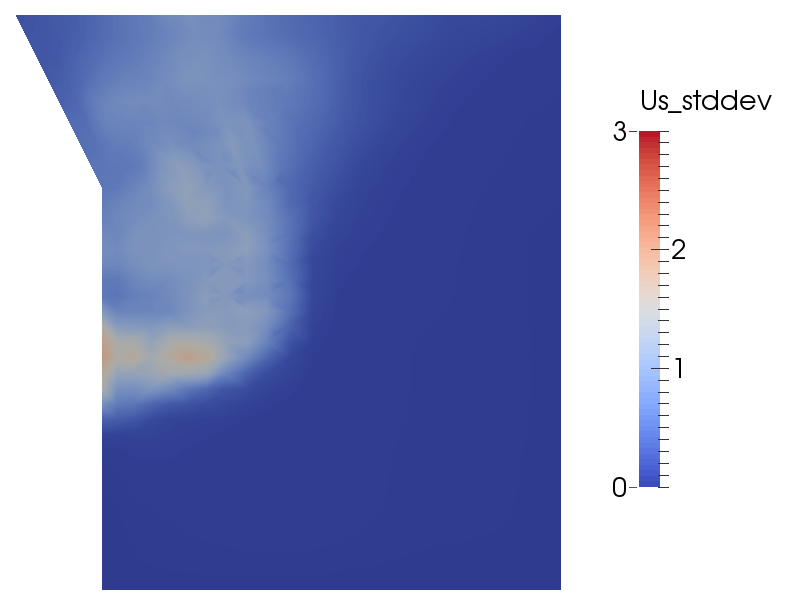
\includegraphics[width=.32\columnwidth]{images/232us_std_hf}
	  \label{fig:232us_std_hf}  }
  \\
  \caption{Particle velocity with different sliding friction coefficient.}
  \label{fig:238racewayus}
\end{sidewaysfigure}
\begin{sidewaysfigure}[htbp]
\centering 
  \subfloat[Low velocity, average void fraction.]
  {
	  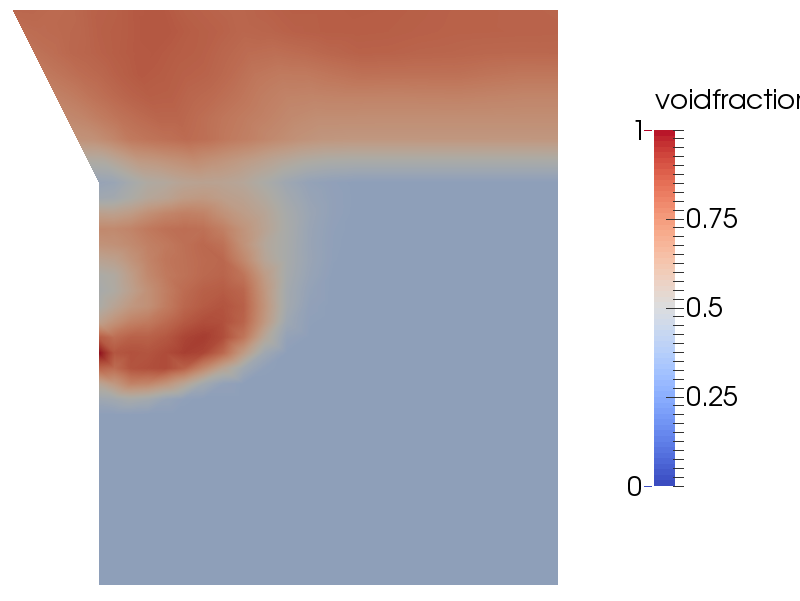
\includegraphics[width=.4\columnwidth]{images/235vf_average_lf}
	  \label{fig:235vf_average_lf}
  }
  \quad
    \subfloat[High friction, average void fraction.]
    {
	  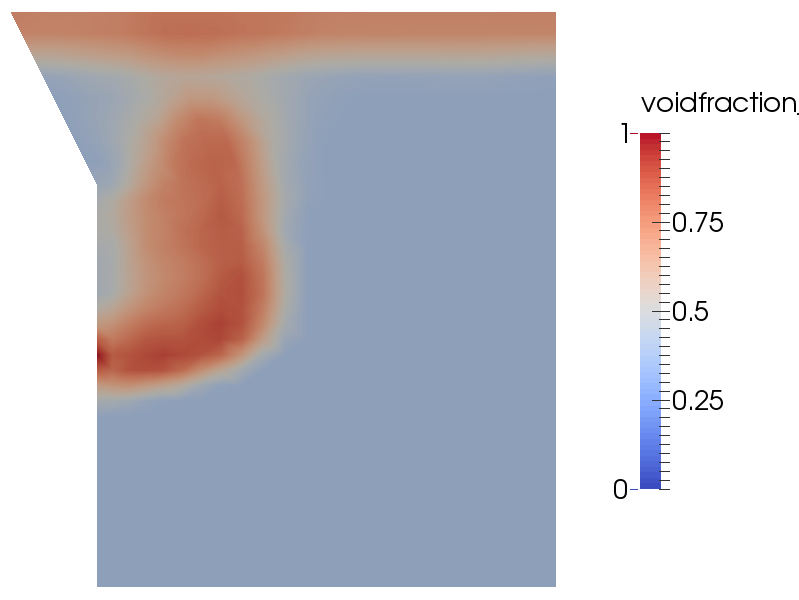
\includegraphics[width=.4\columnwidth]{images/234vf_average_hf}
	  \label{fig:234vf_average_hf}
  }
  \\
  \subfloat[Low velocity, standard deviation void fraction.]
  {
	  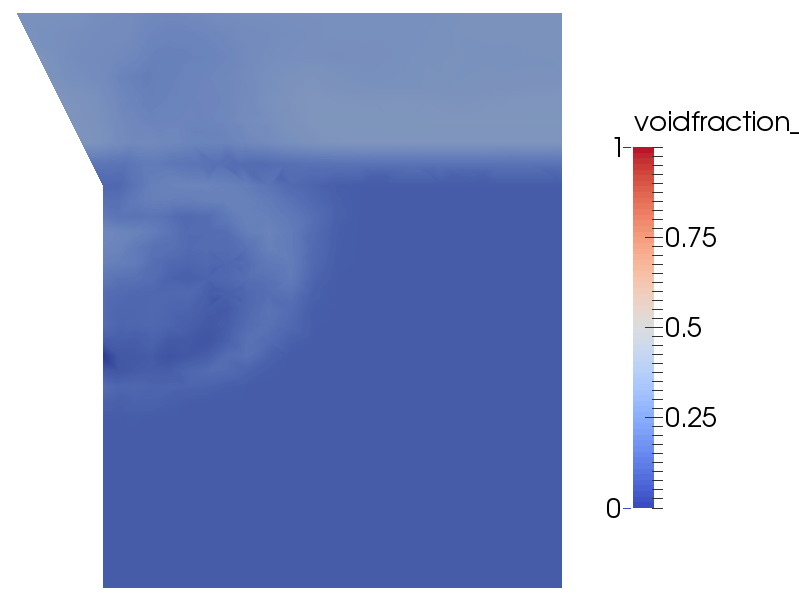
\includegraphics[width=.4\columnwidth]{images/237vf_std_lf}
	  \label{fig:237vf_std_lf}
  }
  \quad
    \subfloat[High friction, standard deviation void fraction.]
    {
	  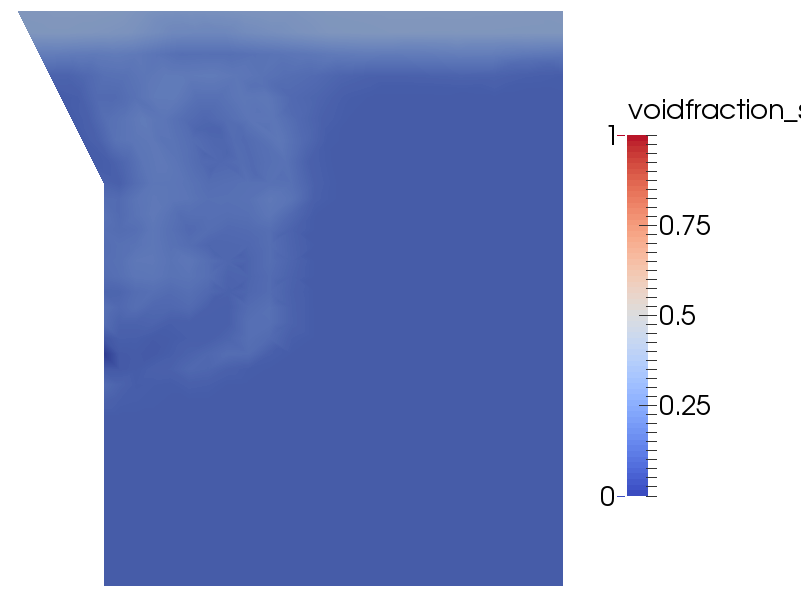
\includegraphics[width=.4\columnwidth]{images/236vf_std_hf}
	  \label{fig:236vf_std_hf}  }
  \\
  \caption{Void fraction with different sliding friction coefficient.}
  \label{fig:239racewayvf}
\end{sidewaysfigure}


% Later, we trained a dedicated \acs{ANN} to evaluate the contribution of each of
% these parameters over the final results.